\chapter{Modeling The Gravitational Potential Of A Small Irregular Body}
\label{gravpot}
\graphicspath{{chapter-2/Images/}}

% Introduction
\section{Introduction}
Before we study the motion of the binary asteroid system or the motion of the spacecraft in the environment of the binary system, it is necessary to define and model the gravitational potential for a small irregular body. Large celestial bodies in the Solar System such as the planets and their moons have, approximately, a spherical shape because the strong gravitational field (due to the large mass of these celestial bodies) has reshaped them into spheres. Unlike the planets and most of their moons, smaller celestial bodies such as asteroids and comets have relatively smaller mass leading to a weaker gravitational field that could not break the material strength to reshape these bodies into spheres. Thus, asteroids and comets are characterized by irregular shapes and consequently an irregular gravitational field \cite{sucarrat_phd}. This chapter will give a brief description on the different ways in which the gravitational potential of a small irregular body can be modeled.

% spherical harmonics gravitational potential
\section{Spherical Harmonics Model}
\label{spherical_harmonics}
Consider a point \textit{P} (see \Cref{fig:spher_harm_init_illustration}), outside a small irregular body (henceforth generalized as an asteroid) corresponding to the position vector \textbf{r} defined as:
\begin{equation}
\label{sph_pos}
\textbf{r} = x\mathbf{\hat{x}} + y\mathbf{\hat{y}} +z\mathbf{\hat{z}}
\end{equation}
%
\begin{figure}[htb]
\centering
\captionsetup{justification=centering}
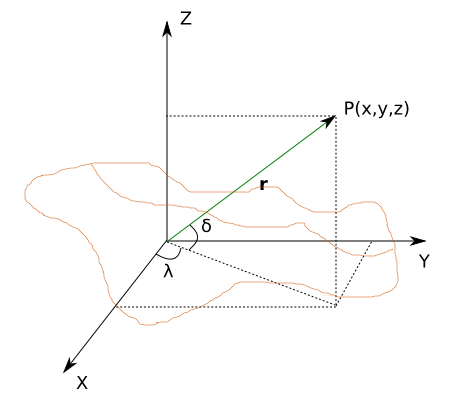
\includegraphics[scale=0.5]{spherical_harmonics_starting_illustration.png}
\caption{Schematic illustrating an irregular body and a point outside this body, denoted as P, where the spherical harmonics potential for the gravity field has to be calculated.}
\label{fig:spher_harm_init_illustration}
\end{figure}

The frame of reference, for all discussions, has its axes aligned with the principal moments of inertia and the origin is at the centre of mass of the body. The spherical coordinates corresponding to \Cref{sph_pos} are defined as \cite{danbook}:
\begin{align}
\label{magn}
r &= \sqrt{x^2 + y^2 + z^2} \\
\label{lat}
\delta &= \sin^{-1}\frac{z}{r} \\
\label{long}
\lambda &= \tan^{-1}\frac{y}{x}
\end{align}
%
where $\delta$ and $\lambda$ are latitude and longitude of the external point, respectively, and $r$ is the magnitude of the position vector. Given the above definitions, the general form for the spherical harmonics gravitational potential is given as \cite{danbook}:
\begin{equation}
\label{sph_harm}
U(r, \delta, \lambda) = \frac{\mu}{r}\sum_{l=0}^{\infty}\sum_{m=0}^{l}\left(\frac{r_0}{r}\right)^lP_{lm}(\sin\delta)[C_{lm}\cos(m\lambda) + S_{lm}\sin(m\lambda)]
\end{equation}
%
Where $\mu = GM$ is the gravitational parameter of the asteroid and $r_0$ is the normalizing radius which is often chosen as the largest radius of the irregularly shaped asteroid or its mean radius  \cite{danbook}. $P_{lm}()$ are the Associated Legendre Function, of degree $l$ and order $m$. $C_{lm}$ and $S_{lm}$ are called the gravity field harmonic coefficients and they describe the dependence of the potential function on a body's internal mass distribution \cite{gillbook} and \cite{danbook}. The Associated Legendre Functions are defined as \cite{kaulabook} and \cite{danbook}:
\begin{align}
\label{legendre}
P_{lm}(\sin\delta) &= \cos^m\delta\sum_{i=0}^{k}T_{lmi}\sin^{l-m-2i}\delta \\
\label{legen_tfunc}
T_{lmi} &= \frac{(-1)^i(2l - 2i)!}{2^li!(l-i)!(l-m-2i)!}
\end{align}
%
where $k$ is the integer part of the term $(l-m)/2$. Explicit formulas for the Associated Legendre Functions upto a degree and order of 2 can be found in \cite{gillbook} (Section 3.2.1, Table 3.1 in \cite{gillbook}). Another method, a recursive method, that is practically used to compute the Associated Legendre functions of any degree (\textit{l}) and order (\textit{m}), with $m<l$, is given as follows \cite{wakker}:
\begin{align}
\label{legendre_zonal_harmonics}
(l+1) P_{(l+1),0}(x) &= (2l+1) x P_{l,0}(x) - l P_{(l-1),0}(x) \\
\label{legendre_sectorial_harmonics}
P_{l,l}(x) &= (2l-1) \sqrt{1-x^2} P_{(l-1),(l-1)}(x) \\
\label{legendre_tesseral_harmonics_1}
P_{l,(l-1)} &= (2l-1) x P_{(l-1),(l-1)}(x) \\
\label{legendre_tesseral_harmonics_2}
P_{l,m}(x) &= \frac{2l-1}{l-m} x P_{(l-1),m}(x) - \frac{l+m-1}{l-m} P_{(l-2),m}(x)
\end{align}
The recursive relations use the starting values $P_{0,0}(x) = 1$ and $P_{1,0}(x) = x$ \cite{wakker}. \Cref{legendre_zonal_harmonics} corresponds to the value of the Associated Legendre Function for the zonal harmonics, \Cref{legendre_sectorial_harmonics} corresponds to the value for the sectorial harmonics, and similarly, \Cref{legendre_tesseral_harmonics_1} and \Cref{legendre_tesseral_harmonics_2} corresponds to the value for the tesseral harmonics \cite{wakker}. The zonal harmonics ($l \neq 0$, $m=0$) in the spherical harmonics potential function for the gravity field, represent the influence of variations in mass density distribution and shape of a body in the north-south direction i.e. the potential changes with the latitude but not with the longitude. The sectorial harmonics ($l = m \neq 0$) represent influence of variation in the mass density and shape of the body in the east-west direction i.e. the potential changes with the longitude but not with the latitude. Finally, the tesseral harmonics ($l \neq m \neq 0$) represent the influence of the variation in mass density and shape of the body in both the east-west and north-south direction i.e. the potential changes with both the latitude and longitude \cite{wakker}. An equation representing the zonal, sectorial and tesseral harmonic parts in the potential function can be found in \cite{wakker} and is not repeated here.
%
\begin{figure}[htb]
\centering
\captionsetup{justification=centering}
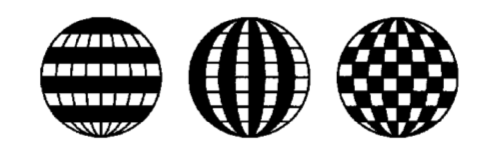
\includegraphics[scale=0.5]{different_spherical_harmonics.png}
\caption{Schematic illustrating the zonal harmonics (left), the sectorial harmonics (centre), and the tesseral harmonics (right) \cite{wakker}.}
\label{fig:different_spherical_harmonics}
\end{figure}

The integral formulas for the gravity coefficients $C_{lm}$ and $S_{lm}$ are given in \cite{gillbook} (see Section 3.2.1, Equation 3.11 in \cite{gillbook}) and also in \cite{danbook} (see Equation 2.15 in \cite{danbook}). The integral expressions for the gravity coefficients are complicated but the solution of the integrals for some lower degree and order cases is well explained in \cite{gillbook} (see Section 3.2.2 in \cite{gillbook}).

\subsubsection{Lower degree and order spherical harmonics gravity field coefficients}
\label{Lower_degree_and_order_coefficients}
%
From the integrand expression for $C_{lm}$ it can easily be evaluated that $C_{00} = 1$. From the integrand expression for $S_{lm}$, we know that all $S_{l0}$ terms will be zero since for $m=0$, the $\sin(m\lambda)$ term in the integral evaluates to zero \cite{gillbook}. The first degree and order gravity coefficients are all related to the centre of mass of the body and the corresponding expressions are given as follows \cite{danbook}:
%
\begin{align}
x_{CM} &= C_{11} r_0 \\
y_{CM} &= S_{11} r_0 \\
z_{CM} &= C_{10} r_0
\end{align}
where $(x_{CM},y_{CM},z_{CM})$ are the coordinates of the centre of mass of the irregular body in the body fixed frame, and $r_0$ is the largest radius or the mean radius of the irregular body. By coinciding the origin of the frame with the centre of the mass i.e. $(x_{CM},y_{CM},z_{CM}) = (0,0,0)$, the three coefficients can be made zero i.e. $C_{11} = S_{11} = C_{10} = 0$. These coefficients however will not be zero if the irregular body does not have a constant density \cite{danbook}.

Now the second degree and order gravity coefficients are related to the body's principle moments of inertia and the products of inertia \cite{danbook}. The ones related to the product of inertia are given as follows \cite{danbook}:
\begin{align}
I_{xy} &= -2M r_0^2 S_{22} \\
I_{yz} &= -M r_0^2 S_{21} \\
I_{xz} &= -M r_0^2 C_{21}
\end{align}
where M is the total mass of the irregular body. By aligning the axes of the body fixed coordinate frame with the principle moments of inertia, the products of inertia become zero, thereby making $S_{22} = S_{21} = C_{21} = 0$.

Thus, the simplest form of the spherical harmonics potential for the gravity field of a body can be defined with only the second degree and order coefficients $C_{20}$ and $C_{22}$. These two coefficients also account for the majority of the gravitational perturbation acting on a dynamical system \cite{danbook}. This simplified gravity potential expression is given as \cite{danbook}:
\begin{equation}
U = \frac{\mu}{r}\left[1 + \left(\frac{r_0}{r}\right)^2\left[C_{20}\left(1-\frac{3}{2}\cos^2\delta\right) + 3C_{22}\cos^2\delta\cos(2\lambda)\right]\right]
\end{equation}

\section{Ellipsoid Harmonics Model}
\label{ellipse_harmonic}
The equation for a fundamental ellipsoid (henceforth called the reference ellipsoid $\varepsilon_0$) is given as \cite{ellipse_main}:
\begin{equation}
\label{fund_ellipse}
\frac{x^2}{a^2} + \frac{y^2}{b^2} + \frac{z^2}{c^2} = 1
\end{equation}
%
where $a \geq b \geq c$ and $a,b,c$ are the semi-major axes of $\varepsilon_0$. Analogous to the Spherical Harmonics, $\varepsilon_0$ will always be the smallest ellipsoid enclosing the entire small irregular body \cite{ellipse_main}. The equation for a family of quadrics, confocal to $\varepsilon_0$ is written as \cite{ellipse_colorado}:
\begin{equation}
\label{hobson_form}
\frac{x^2}{a^2 + s^2} + \frac{y^2}{b^2 + s^2} + \frac{z^2}{c^2 + s^2} = 1
\end{equation}
%
where \textit{s} in \Cref{hobson_form} is a variable; by changing its value a family of quadrics (ellipsoid, hyperboloid of one sheet, or hyperboloid of two sheets \cite{elliptic_integral}) can be generated that will have the same foci as $\varepsilon_0$. Lets define $h, k$ which are two constants such that $0<h<k$ and introduce a change of variable called $\lambda$:
\begin{align}
\label{h_eqn}
h^2 &= a^2 - b^2\\
\label{k_eqn}
k^2 &= a^2 - c^2\\
\label{lambda_general}
\lambda^2 &= a^2 + s^2
\end{align}
%
The quantities $h,k$ are two focal lengths of $\varepsilon_0$. In light of the new terms and their definitions, \Cref{hobson_form} can be re-written as:
\begin{equation}
\label{quadric_family}
\frac{x^2}{\lambda^2} + \frac{y^2}{\lambda^2 - h^2} + \frac{z^2}{\lambda^2 - k^2} = 1
\end{equation}
%
\Cref{quadric_family} has three real roots denoted as $\lambda_1^2, \lambda_2^2, \lambda_3^2$, where $\lambda_1, \lambda_2, \lambda_3$ are called ellipsoidal coordinates. The latter are related to the Cartesian coordinates by the following relations \cite{ellipse_colorado}:
\begin{align}
\label{cart2ellip_x}
x^2 &= \frac{\lambda_1^2 \lambda_2^2 \lambda_3^2}{h^2k^2}\\
\label{cart2ellip_y}
y^2 &= \frac{(\lambda_1^2 - h^2)(\lambda_2^2 - h^2)(h^2 - \lambda_3^2)}{h^2(k^2-h^2)}\\
\label{cart2ellip_z}
z^2 &= \frac{(\lambda_1^2 - k^2)(k^2 - \lambda_2^2)(k^2 - \lambda_3^2)}{k^2(k^2 - h^2)}
\end{align}
%
Because the Cartesian coordinates are related to the ellipsoidal coordinates in a square power, there will be 8 cartesian points corresponding to the same values of $\lambda_1^2, \lambda_2^2, \lambda_3^2$. In order to have a one to one relation between the cartesian and ellipsoidal coordinates, certain restrictions have to be imposed which are provided in \cite{ellipse_colorado} (section 1.1).

Consider a small irregular asteroid body enclosed by the smallest possible reference ellipsoid $\varepsilon_0$ which has a largest semi-major axis denoted by $\lambda_1^{ref}$. Then the potential for the interior space of the ellipsoid is given as follows \cite{ellipse_colorado}:
\begin{equation}
\label{ellipse_internal}
U(\lambda_1, \lambda_2, \lambda_3) = \mu \sum_{n=0}^{\infty} \sum_{p=1}^{2n+1} \alpha_{np} \frac{E_n^p(\lambda_1)}{E_n^p(\lambda_1^{ref})} E_n^p(\lambda_2) E_n^p(\lambda_3)
\end{equation}
%
such that $\lambda_1 \leq \lambda_1^{ref}$. \Cref{ellipse_internal} is also called as the Surface Ellipsoidal Harmonics expansion. In \Cref{ellipse_internal}, $n$ and $p$ define the degree and order, respectively, of the potential expansion; $\mu$ defines the gravitational parameter of the small irregular asteroid body; $\alpha_{np}$ is called the Ellipsoidal Harmonic Coefficient; $E_n^p$ are called Lam\' e's function of the first kind. The latter are divided into four types, defined as follows \cite{ellipse_colorado}:
\begin{align}
\label{lame's_K}
K_n^p(\lambda_i) = a_{0p}\lambda_i^n + a_{1p}\lambda_i^{n-2} + ... +
\left\{
		\begin{aligned}
		& a_{\sigma p} \colon \text{ for n even}\\
		& a_{\sigma p}\lambda_i \colon \text{ for n odd}
		\end{aligned}
\right\}\\
\label{lame's_L}
L_n^p(\lambda_i) = \sqrt{\abs{\lambda_i^2 - h^2}} \times \left[b_{0p}\lambda_i^{n-1} + b_{1p}\lambda_i^{n-3} + ... +
\left\{
		\begin{aligned}
		& b_{n-\sigma -1, p}\lambda_i \colon \text{ for n even}\\
		& b_{n-\sigma -1, p} \colon \text{ for n odd}
		\end{aligned}
\right\}\right]\\
\label{lame's_M}
M_n^p(\lambda_i) = \sqrt{\abs{\lambda_i^2 - k^2}} \times \left[c_{0p}\lambda_i^{n-1} + c_{1p}\lambda_i^{n-3} + ... +
\left\{
		\begin{aligned}
		& c_{n-\sigma -1, p}\lambda_i \colon \text{ for n even}\\
		& c_{n-\sigma -1, p} \colon \text{ for n odd}
		\end{aligned}
\right\}\right]\\
\label{lame's_N}
N_n^p(\lambda_i) = \sqrt{\abs{(\lambda_i^2 - h^2)(\lambda_i^2 - k^2)}} \times \left[d_{0p}\lambda_i^{n-2} + d_{1p}\lambda_i^{n-4} + ... +
\left\{
		\begin{aligned}
		& d_{\sigma -1, p} \colon \text{ for n even}\\
		& d_{\sigma -1, p}\lambda_i \colon \text{ for n odd}
		\end{aligned}
\right\}\right]
\end{align}
%
where $i = 1, 2, 3$ and signifies the index number for the three ellipsoidal coordinates; $K,L,M,N$ are the four types of Lam\' e's function of first kind; $a_{0p}, a_{1p},..., b_{0p}, b_{1p},..., c_{0p}, c_{1p},..., d_{0p}, d_{1p}$ are the polynomial coefficients and:
\begin{equation}
\label{lame_sigma}
\sigma = \left\{
				\begin{aligned}
				& \frac{n}{2} \colon \text{ for n even}\\
				& \frac{n-1}{2} \colon \text{ for n odd}
				\end{aligned}
		\right\}
\end{equation}
%
For a given value for the degree of expansion, $n$, the $E_n^p$ is shared among the four types of Lam\' e's function in the following manner \cite{ellipse_colorado}:
\begin{itemize}
\item $(\sigma + 1)$ are of type $K$ for $p = 1,...,(\sigma + 1)$\\
\item $(n-\sigma)$ are of type $L$ for $p = (\sigma+2),...,(n+1)$\\
\item $(n-\sigma)$ are of type $M$ for $p = (n+2),...,(2n-\sigma+1)$\\
\item $\sigma$ are of type $N$ for $p = (2n-\sigma+2),...,(2n+1)$
\end{itemize}
Thus depending on what the value of the order, $p$, is at a given instant of evaluation in \Cref{ellipse_internal}, the appropriate type of Lam\' e's function is chosen for the term $E_n^p$.
\\
In a similar way, the potential outside the ellipsoid $\lambda_1 = \lambda_1^{ref}$ is defined as \cite{ellipse_colorado}:
\begin{equation}
\label{ellipse_out}
U(\lambda_1, \lambda_2, \lambda_3) = \mu \sum_{n=0}^{\infty} \sum_{p=1}^{2n+1} \alpha_{np} \frac{F_n^p(\lambda_1)}{F_n^p(\lambda_1^{ref})} E_n^p(\lambda_2) E_n^p(\lambda_3) \text{,    } \forall \text{ }\lambda_1 \geq \lambda_1^{ref}
\end{equation}
%
where $F_n^p$ is Lam\' e's function of the second kind and all other terms have the same meaning as defined earlier for \Cref{ellipse_internal}. $F_n^p$ is defined as follows \cite{ellipse_colorado}:
\begin{equation}
\label{Lame's_F}
F_n^p(\lambda_1) = (2n+1) E_n^p(\lambda_1) \int_{\lambda_1}^{\infty} \frac{du}{(E_n^p(u))^2 \sqrt{(u^2-k^2)(u^2-h^2)}}
\end{equation}
%
where $u$ is just an integration variable. Of course at the boundary $\lambda_1 = \lambda_1^{ref}$, \Cref{ellipse_internal} and \Cref{ellipse_out} have the same expression so that the potential is continuous \cite{ellipse_colorado}.
\\
It is often preferred to use a normalized expression for a gravitational potential, mainly because normalization helps to simplify these expressions and avoids combination of large and small numerical quantities in computations, such as multiplication. The normalization constant (the use of the normalization constant is shown in \Cref{bar1} and \Cref{bar2}) is shown here without any derivation \cite{ellipse_colorado}:
\begin{equation}
\label{ellipse_norm}
\gamma_n^p = 8 \times \int_{0}^{h} \int_h^k \frac{(\lambda_2^2 - \lambda_3^2)(E_n^p(\lambda_2)E_n^p(\lambda_3))^2}{\sqrt{(k^2-\lambda_2^2)(\lambda_2^2-h^2)(h^2-\lambda_3^2)(k^2-\lambda_3^2)}}d\lambda_2d\lambda_3
\end{equation}
%
Thus the normalized ellipsoidal harmonic expansion of the gravitational potential are expressed as:
\begin{align}
\label{ellipse_norm_in}
U(\lambda_1, \lambda_2, \lambda_3) &= \mu \sum_{n=0}^{\infty} \sum_{p=1}^{2n+1} \overline{\alpha_{np}} \frac{E_n^p(\lambda_1)}{E_n^p(\lambda_1^{ref})} \overline{E_n^p(\lambda_2)} \text{ } \overline{E_n^p(\lambda_3)}  \text{,    } \forall \text{ }\lambda_1 \leq \lambda_1^{ref} \\
\label{ellipse_norm_out}
U(\lambda_1, \lambda_2, \lambda_3) &= \mu \sum_{n=0}^{\infty} \sum_{p=1}^{2n+1} \overline{\alpha_{np}} \frac{F_n^p(\lambda_1)}{F_n^p(\lambda_1^{ref})} \overline{E_n^p(\lambda_2)} \text{ } \overline{E_n^p(\lambda_3)} \text{,    } \forall \text{ }\lambda_1 \geq \lambda_1^{ref} \\
\label{bar1}
\overline{E_n^p(\lambda_2)} \text{ } \overline{E_n^p(\lambda_3)} &= \frac{E_n^p(\lambda_2) E_n^p(\lambda_3)}{\sqrt{\gamma_n^p}}\\
\label{bar2}
\overline{\alpha_{np}} &= \alpha_{np} \sqrt{\gamma_n^p}
\end{align}
%
The ellipsoidal harmonic coefficient $\alpha_{np}$ can be expressed as a linear transformation of the spherical harmonics coefficients $C_{lm}$ and $S_{lm}$ as follows \cite{ellipse_colorado}:
\begin{equation}
\label{alpha_coeff}
\overline{\alpha_{np}} = \sum_{l=0}^{\infty} \sum_{m=0}^{l} (A_{np}^{lm}.C_{lm} + B_{np}^{lm}.S_{lm})
\end{equation}
%
where $l$ and $m$ represent the degree and order from the spherical harmonic expansion; $A_{np}^{lm}$ and $B_{np}^{lm}$ represent the transformation coefficients. Depending on the type (even or odd) of $l,m,n,p$, the various values of the transformation coefficients are given in reference \cite{ellipse_colorado} (section 2.3.2.2) which shall be used in the computation of the ellipsoidal harmonic expansion of the gravitational potential for an irregularly shaped asteroid body.

\section{Elliptic Integral Model}
\label{elliptic_integral}
Before we can begin with the expressions for the gravitational potential for an elliptic integral, we will have to revisit the theory of ellipsoidal coordinates. This is necessary since the theory shall be presented in a different manner compared to that in \Cref{ellipse_harmonic} because unlike in that section, the theory presented here shall result in the formulation of a one-to-one relation between cartesian and ellipsoidal coordinates without the involvement of external conditions or restrictions. The theory for this section has mainly been derived from a previous research work given in \cite{elliptic_integral} and the reader is strongly advised to refer \cite{elliptic_integral} for more details.
\begin{equation}
\label{hobson_form_2}
\frac{x^2}{a^2 + s^2} + \frac{y^2}{b^2 + s^2} + \frac{z^2}{c^2 + s^2} = 1
\end{equation}
%
\Cref{hobson_form_2} is a cubic equation ($a \geq b \geq c$) in $s$ and has three unequal real roots in $s$ denoted here as $s_1, s_2, s_3$. The latter are also called ellipsoidal coordinates as described in \cite{elliptic_integral}. Note that the form of ellipsoidal coordinates mentioned here as $s_1, s_2, s_3$ is not the same as that of $\lambda_1, \lambda_2, \lambda_3$  mentioned in \Cref{ellipse_harmonic}. The three pairs of foci of the triaxial ellipsoid $\varepsilon_0$ (circumscribing ellipsoid for an irregular body) are denoted as $(\pm E_x, 0, 0)$, $(\pm E_e, 0, 0)$, $(\pm E_y, 0, 0)$ and can be seen in \Cref{xzplane}, \Cref{yzplane}, and \Cref{xyplane}. In the same figures, the reader can also notice the semi-major axes $a,b,c$ of $\varepsilon_0$. These figures are a much simplified diagram (and also not to scale), depicting the ellipsoid and its parameters, compared to the ones rendered in \cite{elliptic_integral} (see section 2 of \cite{elliptic_integral}).

\begin{figure}[h]
\centering
\captionsetup{justification=centering}
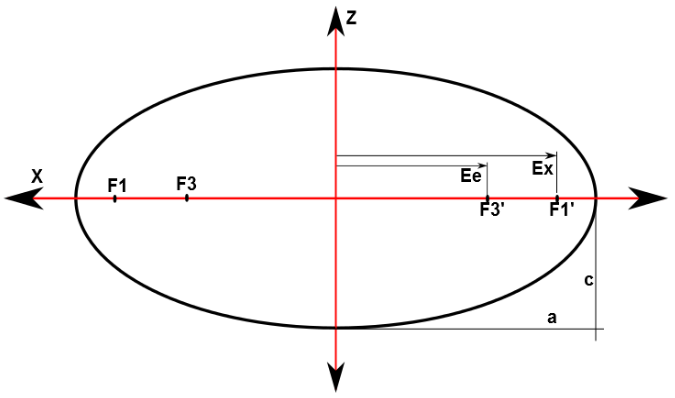
\includegraphics[scale=0.5]{ellipse_1_final.png}
\caption{$X-Z$ plane of triaxial ellipsoid.}
\label{xzplane}
\end{figure}
%
\begin{figure}[h]
\centering
\captionsetup{justification=centering}
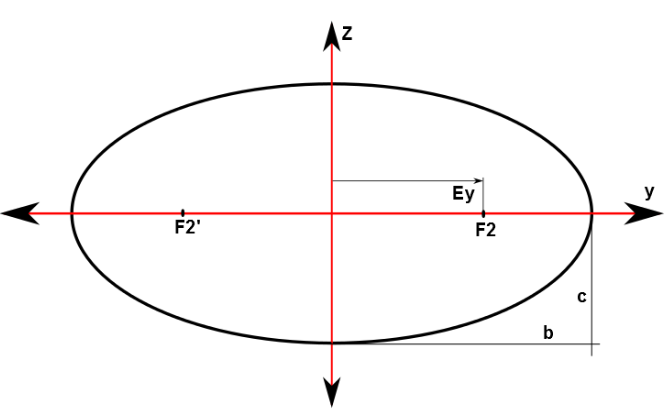
\includegraphics[scale=0.5]{ellipse_2_final.png}
\caption{$Y-Z$ plane of triaxial ellipsoid.}
\label{yzplane}
\end{figure}
%
The focal lengths are given as $E_x = \sqrt{a^2 - c^2}$, $E_y = \sqrt{b^2 - c^2}$, and $E_e = \sqrt{a^2 - b^2}$. The parameter $E_e$ can be related to $E_x$ and $E_y$ as $E_e^2 = E_x^2 - E_y^2$ \cite{elliptic_integral}. The general relation between the ellipsoidal coordinates ($s_1, s_2, s_3$) and the cartesian coordinates ($x,y,z$) is given as \cite{elliptic_integral}:
\begin{align}
\label{xsrel}
x^2 &= \frac{(a^2 + s_1)(a^2 + s_2)(a^2+s_3)}{(a^2-b^2)(a^2-c^2)}\\
\label{ysrel}
y^2 &= \frac{(b^2 + s_1)(b^2 + s_2)(b^2+s_3)}{(b^2-a^2)(b^2-c^2)}\\
\label{zsrel}
z^2 &= \frac{(c^2 + s_1)(c^2 + s_2)(c^2+s_3)}{(c^2-a^2)(c^2-b^2)}
\end{align}
%
\begin{figure}[h]
\centering
\captionsetup{justification=centering}
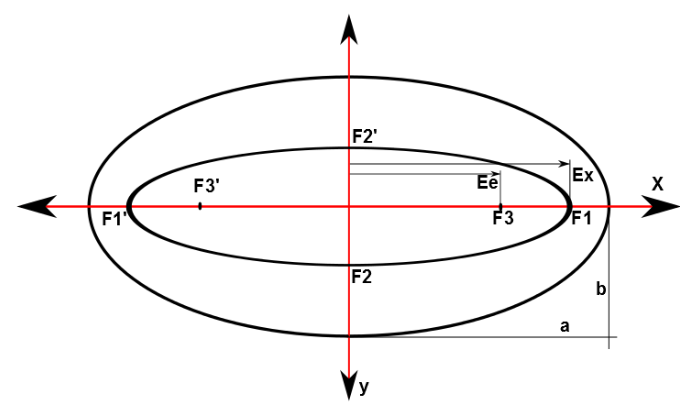
\includegraphics[scale=0.5]{ellipse_3_final.png}
\caption{$X-Y$ plane of triaxial ellipsoid.}
\label{xyplane}
\end{figure}
%
The transformation given in \Cref{xsrel}, \Cref{ysrel}, and \Cref{zsrel} is not one-to-one and for each ellipsoidal coordinate ($s_1, s_2, s_3$) there exists eight cartesian points ($\pm x,\pm y,\pm z$). \cite{elliptic_integral} has introduced an alternate variant of ellipsoidal coordinates so as to have a one to one relation with the cartesian coordinates. These new ellipsoidal coordinates will be denoted as ($u, \beta, \lambda$) and are given by the following relations:
\begin{align}
\label{uelip}
s_1 &= u^2 - c^2\\
\label{betaelip}
s_2 &= -b^2\sin^2(\beta) - c^2\cos^2(\beta)\\
\label{lambdaelip}
s_3 &= -a^2\sin^2(\lambda)-b^2\cos^2(\lambda)
\end{align}
%
In the new ellipsoidal coordinates ($u, \beta, \lambda$), $u$ is the polar semi-axis of the ellipsoid, $\beta$ is the ellipsoidal latitude and $\lambda$ is the ellipsoidal longitude \cite{elliptic_integral}. Upon substituting \Cref{uelip}, \Cref{betaelip}, and \Cref{lambdaelip} into \Cref{xsrel}, \Cref{ysrel}, and \Cref{zsrel}, the following relations are obtained \cite{elliptic_integral}:
\begin{align}
\label{xelip}
x &= \sqrt{u^2 + E_x^2} \left[\cos^2\beta + \frac{E_e^2}{E_x^2}\sin^2\beta \right]^{1/2} \cos\lambda\\
\label{yelip}
y &= \sqrt{u^2 + E_y^2}\cos\beta \sin\lambda\\
\label{zelip}
z &= u\sin\beta \left[1 - \frac{E_e^2}{E_x^2}\cos^2\lambda \right]^{1/2}
\end{align}
%
where $u \geq 0$, $-\pi/2 \leq \beta \leq \pi/2$, and $-\pi < \lambda \leq \pi$. \Cref{xelip} to \Cref{zelip} show a one to one correspondence between the cartesian coordinates and the alternate variant of ellipsoidal coordinates. Now that we have developed an understanding for the ellipsoidal coordinates, we shall discuss the expression for the gravitational potential of a triaxial ellipsoid given in terms of an elliptic integral.
\\\\
The gravitational potential U of a homogeneous ellipsoid can be expressed in terms of an integral as follows \cite{elliptic_integral}:
\begin{equation}
\label{elliptic_pot}
U(s_1, s_2, s_3) = \frac{3}{4} \mu \int_{s_1}^{\infty} \left[1 - \frac{x^2}{a^2+s} - \frac{y^2}{b^2+s} - \frac{z^2}{c^2+s} \right] \frac{ds}{\sqrt{(a^2+s)(b^2+s)(c^2+s)}}
\end{equation}
%
where $(s_1, s_2, s_3)$ are the ellipsoidal coordinates which are related to the Cartesian coordinates by \Cref{xsrel}, \Cref{ysrel} and \Cref{zsrel}. In terms of the alternate variant of ellipsoidal coordinates, $(u, \beta, \lambda)$, the gravitational potential is expressed as \cite{elliptic_integral}:
\begin{equation}
\label{elliptic_altpot}
U(u,\beta,\lambda) = \frac{3}{2} \mu \int_{u}^{\infty} \left[1 - \frac{x^2}{\sigma^2+E_x^2} - \frac{y^2}{\sigma^2+E_y^2} - \frac{z^2}{\sigma^2} \right] \frac{d\sigma}{\sqrt{(\sigma^2+E_x^2)(\sigma^2+E_y^2)}}
\end{equation}
%
The expression in \Cref{elliptic_altpot} can further be broken down into four "basic" integrals \cite{elliptic_integral}:
\begin{equation}
\label{elliptic_altpot_expand}
U(u,\beta,\lambda) = \frac{3}{2} \mu (I_0(u) - x^2I_1(u) - y^2I_2(u) - z^2I_3(u))
\end{equation}
%
where
\begin{align}
\label{I0}
I_0(u) &= \int_u^{\infty} \frac{d\sigma}{\sqrt{(\sigma^2+E_x^2)(\sigma^2+E_y^2)}} \\
\label{I1}
I_1(u) &= \int_u^{\infty} \frac{d\sigma}{\sqrt{(\sigma^2+E_x^2)^3(\sigma^2+E_y^2)}} \\
\label{I2}
I_2(u) &= \int_u^{\infty} \frac{d\sigma}{\sqrt{(\sigma^2+E_x^2)(\sigma^2+E_y^2)^3}} \\
\label{I3}
I_3(u) &= \int_u^{\infty} \frac{d\sigma}{\sigma^2 \sqrt{(\sigma^2+E_x^2)(\sigma^2+E_y^2)}}
\end{align}
%
\Cref{elliptic_altpot_expand}, at first look, does not seem to have any dependency on the ellipsoidal coordinates $u,\beta,\lambda$ but the dependence becomes apparent when the $x,y,z$ coordinates are substituted from \Cref{xelip} to \Cref{zelip} into \Cref{elliptic_altpot_expand}. The integrals $I_0, I_1, I_2$, and $I_3$ can be expressed as elliptic integrals of the first and the second kind in order to be evaluated. However these integrals can also be computed using numerical integration methods. In order to use the numerical method, these improper integrals (since they are definite integral with one of the boundaries being $\infty$) have to be converted into proper definite integrals by applying the transformation $\sigma = 1/t$ (note that the lower and upper boundaries of the new integrals change because of applying the transformation). The transformed integrals are shown below \cite{elliptic_integral}:
\begin{align}
\label{I0t}
I_0(u) &= \int_0^{1/u} \frac{dt}{\sqrt{(1+E_x^2 t^2)(1 + E_y^2 t^2)}} \\
\label{I1t}
I_0(u) &= \int_0^{1/u} \frac{t^2 dt}{\sqrt{(1+E_x^2 t^2)^3(1 + E_y^2 t^2)}} \\
\label{I2t}
I_0(u) &= \int_0^{1/u} \frac{t^2 dt}{\sqrt{(1+E_x^2 t^2)(1 + E_y^2 t^2)^3}} \\
\label{I3t}
I_0(u) &= \int_0^{1/u} \frac{t^2 dt}{\sqrt{(1+E_x^2 t^2)(1 + E_y^2 t^2)}}
\end{align}
%
Thus using any numerical integration method, \Cref{I0t} to \Cref{I3t} can be computed which can then be utilized in \Cref{elliptic_altpot_expand} to compute the gravitational potential at any given point $x,y,z$ external to the ellipsoid.

\section{Mass Concentration Model}
\label{mascon}
To calculate the trajectory of a particle around a single or a system of small irregularly shaped bodies, the mass concentrations or \textit{"mascon"} model can also be used. In this method, the entire volume of the small irregular body can be filled with a uniform grid of point masses such that the sum of all these point masses equals the total mass of the body. The acceleration for a particle or spacecraft in orbit around such a small irregular body is then calculated as a vector sum of accelerations due to each point mass. The position and velocity of the particle in orbit and that of the rotating small irregular body are then updated in each time step \cite{mascon}. \\\\
Consider $m_i$ being one of the point masses in the distribution where $i = 1,..., n$ and $n$ is the total number of point masses; $U_i$ being the gravitational potential due to the point mass $i$; $\mathbf{r_i}$ being the Cartesian position vector of the orbiting particle from the point mass $i$ in the inertial reference frame; $a_i$ being the acceleration due to the point mass $i$; then the following relations can be written:
\begin{align}
U_i &= \frac{Gm_i}{r_i} \\
\overrightarrow{a_i} &= \frac{\delta}{\delta x} (U_i) \hat{x} + \frac{\delta}{\delta y} (U_i) \hat{y} + \frac{\delta}{\delta z} (U_i) \hat{z}
\end{align}
%
The total acceleration will then be given as:
\begin{equation}
\overrightarrow{a_{tot}} = \sum_{i=1}^n \overrightarrow{a_i}
\end{equation}
%

\section{Polyhedron Model}
\label{polyhedron}
A polyhedron is a three-dimensional solid body whose surface consists of several planar faces (or facets) that meet along straight edges or at isolated points called vertices. An edge can be common to only two faces. These planar faces are, in general, polygons. Three or more of these planar faces meet at each vertex. The reader should note that just the vertex coordinates alone are not sufficient enough to completely describe a polyhedron. In addition to the vertex coordinates, information about which edge connects which vertex pair and bounds which face pair should also be given to completely characterize a polyhedron. To adopt the polyhedron modeling of gravitational attraction, two important assumptions are made \cite{dan_poly}:
\begin{itemize}
\item The asteroid is a polyhedron
\item The asteroid's density is constant
\end{itemize}
%
Each polyhedron face has a normal vector $\hat{n}_f$, which is pointing outwards, and a face dyad $F_f = \hat{n}_f\hat{n}_f$. The latter is basically a dyadic product of the normal vector with itself. Now each edge of each face also has its own normal vector denoted as $\hat{n}_e^f$ which is perpendicular to $\hat{n}_f$ and also to the edge to which it belongs. This edge normal vector lies in the plane of the corresponding face \cite{dan_poly}. \Cref{fig:poly_face} gives a graphical view of the different vectors just described. For the common edge $P1P2$ connecting faces A and B (see \Cref{fig:poly_face}) the edge dyad is defined as $E_{12} = \hat{n}_A \hat{n}_{12}^A + \hat{n}_B\hat{n}_{21}^B$ i.e. the summation of two dyadic products. Other edge dyads, $E_e$, are defined in a similar way \cite{dan_poly}.
%
\begin{figure}[h]
\centering
\captionsetup{justification=centering}
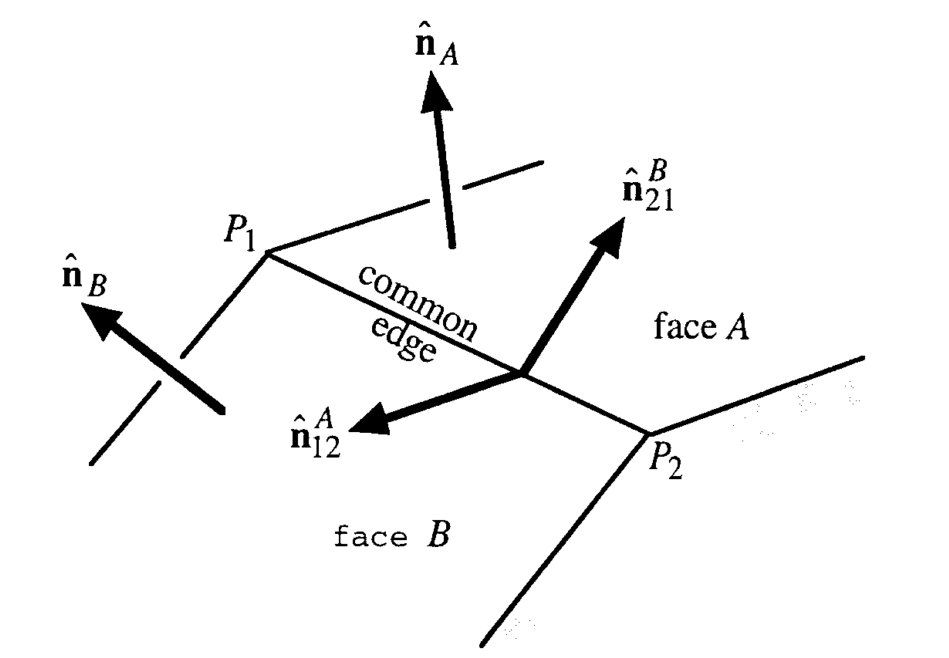
\includegraphics[scale=0.5]{poly_faces.png}
\caption{Two adjacent faces of the polyhedron depicting the common edge P1P2. $\hat{n}_A$ and $\hat{n}_B$ are the two face normal vectors; $\hat{n}_{12}^A$ and $\hat{n}_{21}^B$ are the edge normal vectors situated in planes A and B respectively \cite{dan_poly}.}
\label{fig:poly_face}
\end{figure}
\FloatBarrier
%
Consider one edge of a face on the polyhedron. Let this edge have two vertex points denoted as $P_i$ and $P_j$. Let the length of the edge be denoted as $e_{ij}$. Consider a point external to the polyhedron, henceforth called as the field point i.e. the point at where the potential is to be calculated. Let the distance vectors from this field point to the vertices $P_i$ and $P_j$ be denoted as $\overrightarrow{r_i}$ and $\overrightarrow{r_j}$ respectively. Then the dimensionless per-edge factor $L_e$ is denoted as \cite{dan_poly}:
\begin{equation}
\label{edgefactor}
L_e = \ln \frac{||\overrightarrow{r_i}|| + ||\overrightarrow{r_j}|| + e_{ij}}{||\overrightarrow{r_i}|| + ||\overrightarrow{r_j}|| - e_{ij}}
\end{equation}
%
Now consider that each face of the polyhedron is triangular, bounded by vertices $P_i$, $P_j$, and $P_k$. Each of these vertices has a position vector defined from a field point external to the polyhedron as $\overrightarrow{r_i}$, $\overrightarrow{r_j}$, and $\overrightarrow{r_k}$ respectively. Then the dimensionless per-face factor $w_f$ is denoted as \cite{dan_poly}:
\begin{equation}
\label{facefactor}
w_f = 2 \arctan \frac{\overrightarrow{r_i} \cdot \overrightarrow{r_j} \times \overrightarrow{r_k}}{||\overrightarrow{r_i}|| \cdot ||\overrightarrow{r_j}|| \cdot ||\overrightarrow{r_k}|| + ||\overrightarrow{r_i}||(\overrightarrow{r_j} \cdot \overrightarrow{r_k}) + ||\overrightarrow{r_j}||(\overrightarrow{r_k} \cdot \overrightarrow{r_i}) + ||\overrightarrow{r_k}||(\overrightarrow{r_i} \cdot \overrightarrow{r_j})}
\end{equation}
%
Using the above definitions, the gravitational potential of a polyhedron at a variable field point can be defined as \cite{dan_poly}:
\begin{equation}
\label{polypot}
U = \frac{1}{2} G \sigma \sum_{e\in edges} \overrightarrow{r}_e \cdot E_e \cdot \overrightarrow{r}_e \cdot L_e - \frac{1}{2} G \sigma \sum_{f\in faces} \overrightarrow{r}_f \cdot F_f \cdot \overrightarrow{r}_f \cdot w_f
\end{equation}
%
The vector $\overrightarrow{r}_e$ is a position vector from the field point to any point on the edge $e$, similarly the vector $\overrightarrow{r}_f$ is the position vector from the field point to any point in the face $f$, G is the universal gravitational constant, and $\sigma$ is the (constant) density of the polyhedron. Thus with the definitions given above, the gravitational potential at any external field point can be easily calculated. An example polyhedron model for the primary asteroid in the binary system 1999 KW4 is shown in \Cref{fig:poly_examp} \cite{stefaan_thesis}.
\begin{figure}[h]
\centering
\captionsetup{justification=centering}
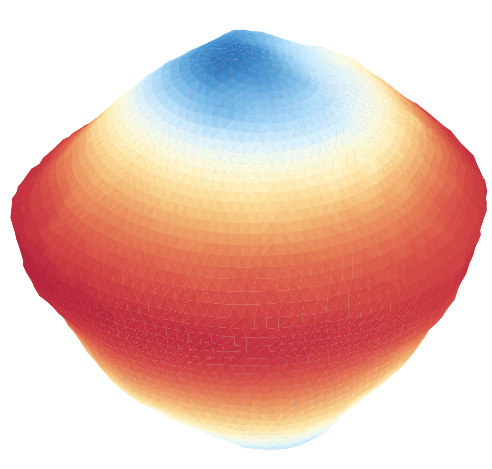
\includegraphics[scale=0.5]{kw4.png}
\caption{polyhedron model of the primary asteroid in binary system 1999 KW4. Red faces indicate higher potential, blue indicate low potential \cite{stefaan_thesis}.}
\label{fig:poly_examp}
\end{figure}
\FloatBarrier
%
\section{Conclusion}
This chapter discussed various methods in which the gravitational potential of a small irregular body (or in general any celestial body) can be modeled. This section will present a subjective discussion (based on certain criteria) on the advantages and/or disadvantages of using any particular model. We will also look into the results from an objective comparison performed between the ellipsoidal harmonics model and the spherical harmonics model, where the polyhedron model was used as the reference. The objective results were taken from a previous study in \cite{spherical_ellipsoidal_comparison}.

The criteria which shall be responsible for deciding the relevance of a given potential model are as follows:
\begin{itemize}
\item Computational economy
\item Volume of divergence
\item Accuracy
\item Availability of physical data on asteroids
\item Application
\end{itemize}
%
The classical approach for modeling the gravitational field for an arbitrary body is in the form of a spherical harmonics expansion. This method involves relatively simple mathematics and converges to an accurate value of the gravity field outside the circumscribing sphere (see \Cref{fig:circum_sphere}). Finite truncation orders can model the potential of the body to have a close match with the "true" potential. To improve the accuracy of the model, for a given body, the spherical harmonic coefficients can be determined with a high accuracy by evaluating the perturbations acting on the orbiting spacecraft. The disadvantage, however, is that the spherical harmonic expansion model exhibits severe divergence within the circumscribing sphere \cite{ellipse_colorado}. The gravitational acceleration using the spherical harmonics model was calculated for the asteroid 433 Eros in \cite{spherical_ellipsoidal_comparison}. The acceleration due to gravity was calculated on a reference circumscribing sphere using the polyhedron model and then again by using the spherical harmonics model. The difference between the two were then calculated to judge the accuracy of the spherical harmonics model for a highly elongated and irregular shape of Eros (the study considered the gravitational acceleration computed using the polyhedron model as the "true" acceleration). The results for the differences in computed gravitational acceleration between the spherical harmonics (degree 10 and 20) and the polyhedron model are shown in \Cref{fig:spherical_10_comparison} and \Cref{fig:spherical_20_comparison} respectively \cite{spherical_ellipsoidal_comparison}. The errors reduce when the degree of the spherical harmonic expansion is increased, indicating that higher orders can provide a very good approximation of the "true" gravity field.
%
\begin{figure}[h]
\begin{minipage}[t]{0.5\textwidth}
\centering
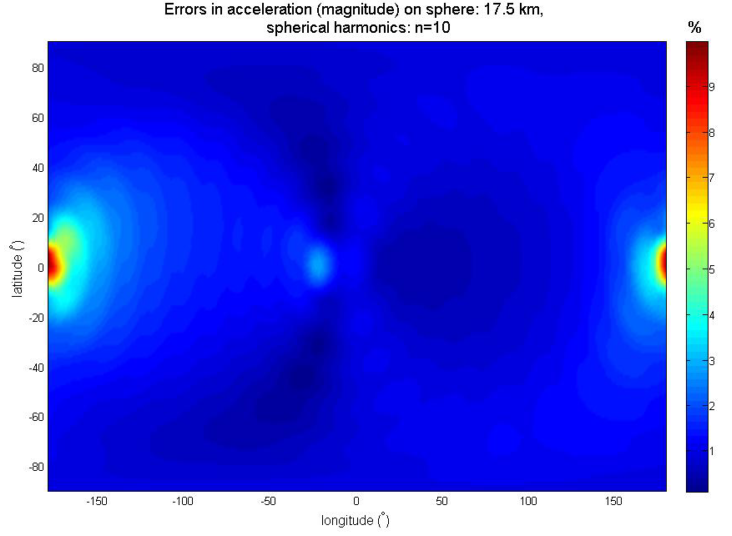
\includegraphics[width=\textwidth]{spherical_10_comparison.png}
\caption{Difference in the computed gravitational acceleration between the spherical harmonics model of degree 10 and the polyhedron model \cite{spherical_ellipsoidal_comparison}.}
\label{fig:spherical_10_comparison}
\end{minipage}
\hspace{0.5cm}
\begin{minipage}[t]{0.5\textwidth}
\centering
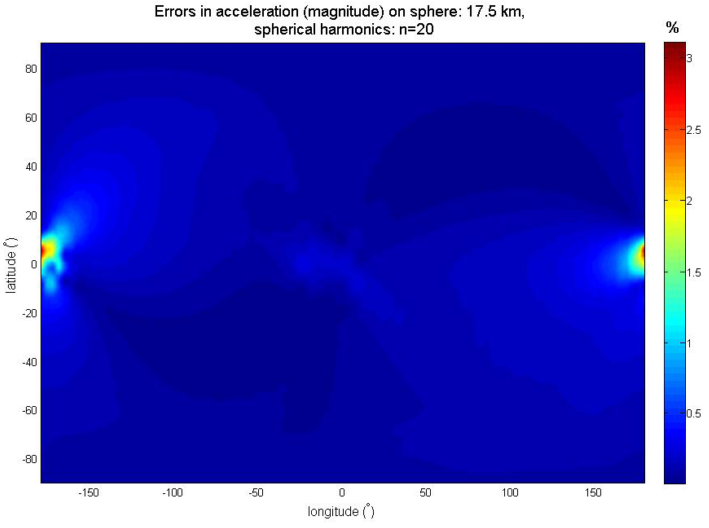
\includegraphics[width=\textwidth]{spherical_20_comparison.png}
\caption{Difference in the computed gravitational acceleration between the spherical harmonics model of degree 20 and the polyhedron model \cite{spherical_ellipsoidal_comparison}.}
\label{fig:spherical_20_comparison}
\end{minipage}
\end{figure}

As explained in \Cref{spherical_harmonics}, that majority of the perturbations from the non-uniform gravitational field of an irregular body can be accounted for by just taking the second degree and order coefficients, however, determining the values for these coefficients can itself be a problem if no spacecraft tracking data around an asteroid is available (from which the values of the coefficients can be determined) or if the principle moments of inertia of the asteroid are unknown. It is easy to infer that if the values for the gravitational coefficients are unknown then the spherical harmonics model can not be used.

For close proximity operations, the spherical harmonics model can not be used to model the gravity of an asteroid since the spherical harmonics expansion diverges inside the circumscribing sphere. In general, the spherical harmonics model is not suitable for aspherical bodies \cite{ellipse_main} since the circumscribing sphere does not provide an optimal fit to such a body leading to large volumes of space around the body where the expansion diverges severely. The circumscribing sphere can be seen in \Cref{fig:circum_sphere}. Thus, although we can increase the accuracy of the gravitational potential modeling by increasing the degree and order of the harmonics expansion, it still can not avoid the divergence of the expansion inside the circumscribing sphere. For applications involving the study of motion on or very close to the surface of an asteroid, such as the orbital motion of lofted regolith, the spherical harmonics model can not be used.
%
\begin{figure}[h]
\centering
\captionsetup{justification=centering}
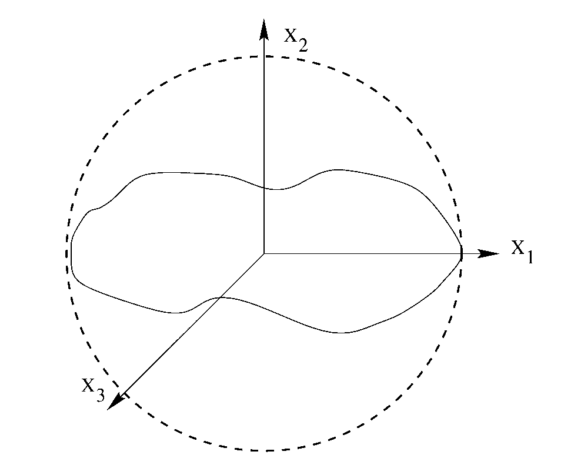
\includegraphics[scale=0.38]{circum_sphere.png}
\caption{Circumscribing sphere (or the Brillouin sphere) \cite{ellipse_main}.}
\label{fig:circum_sphere}
\end{figure}
\FloatBarrier
%

We shall now evaluate the feasibility of using the ellipsoidal harmonics expansion. The difference in the computed gravitational acceleration, for 433 Eros, between the ellipsoidal harmonics model, of degrees 10 and 20, and the polyhedron model is shown in \Cref{fig:ellipsoidal_10_comparison} and \Cref{fig:ellipsoidal_20_comparison}. The accelerations were calculated on the reference ellipsoid that circumscribed Eros \cite{spherical_ellipsoidal_comparison}. Note that the peak value for the difference in the degree 10 expansion case is more than that of the corresponding spherical harmonics case. The order of magnitude for the difference in the gravitational accelerations for the degree 20 expansion of the ellipsoidal harmonics is, however, the same as that for the corresponding spherical harmonics expansion. Just like in the case of the spherical harmonics, by increasing the degree of the ellipsoidal harmonics expansion, the accuracy of the modeled gravitational field has increased. For irregular and elongated bodies such as Eros, \cite{spherical_ellipsoidal_comparison} mentions that the spherical harmonics expansion is less suitable than the ellipsoidal harmonics expansion.
%
\begin{figure}[h]
\begin{minipage}[t]{0.5\textwidth}
\centering
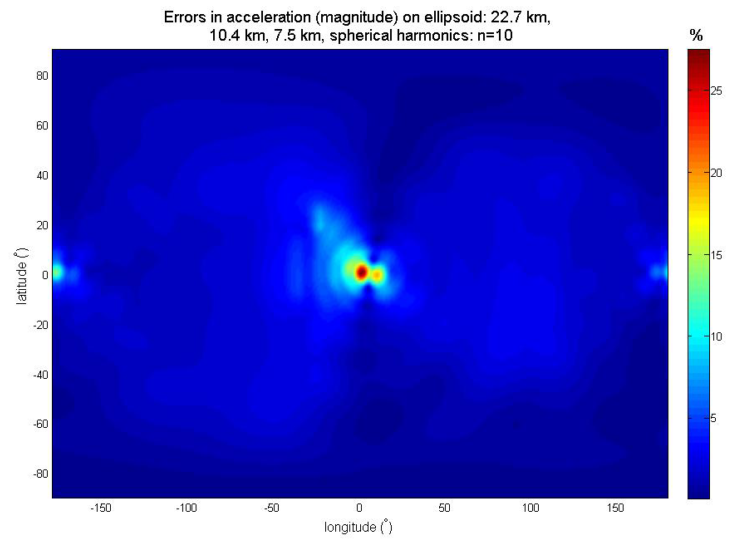
\includegraphics[width=\textwidth]{ellipsoidal_10_comparison.png}
\caption{Difference in the computed gravitational acceleration between the ellipsoidal harmonics model of degree 10 and the polyhedron model \cite{spherical_ellipsoidal_comparison}.}
\label{fig:ellipsoidal_10_comparison}
\end{minipage}
\hspace{0.5cm}
\begin{minipage}[t]{0.5\textwidth}
\centering
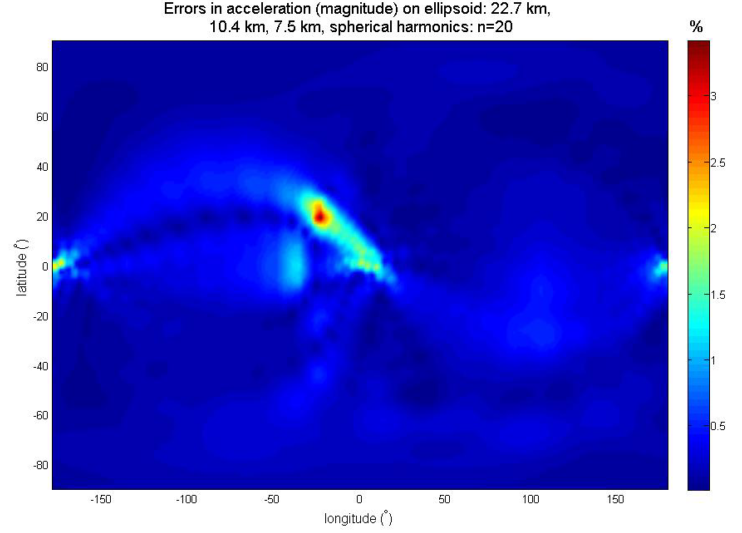
\includegraphics[width=\textwidth]{ellipsoidal_20_comparison.png}
\caption{Difference in the computed gravitational acceleration between the ellipsoidal harmonics model of degree 20 and the polyhedron model \cite{spherical_ellipsoidal_comparison}.}
\label{fig:ellipsoidal_20_comparison}
\end{minipage}
\end{figure}

Just like in the case of the spherical harmonics expansion, the ellipsoidal harmonic expansion is convergent outside the circumscribing ellipsoid or the Brillouin ellipsoid. For an irregular body, an ellipsoid fits more closely rather than a sphere (see \Cref{fig:circum_ellip}), and thus the volume of divergence of the ellipsoidal harmonic expansion is reduced. This provides an opportunity to work with orbits around an asteroid at close proximity. Again due to the fact that an ellipsoid can fit an irregular body more closely than a sphere, the potential calculated at a point close to the body is much accurate in the case of ellipsoidal harmonic expansion rather than the spherical harmonic expansion \cite{ellipse_main}. Within their respective volumes of divergence, the ellipsoidal harmonics model performs better than its spherical counterpart \cite{spherical_ellipsoidal_comparison}. This is evident from \Cref{fig:surface_comparison_spherical_ellipsoidal}. It illustrates the difference in the computed gravitational potential for Phobos between the polyhedron model and the two harmonic (spherical and ellipsoidal) expansion models \cite{spherical_ellipsoidal_comparison}. The performance of the ellipsoidal harmonics model is much better than that of the spherical harmonics, within their respective volume of divergence. Note that the points at which the potential was calculated in both cases, was the same \cite{spherical_ellipsoidal_comparison}.
%
\begin{figure}[h]
\centering
\captionsetup{justification=centering}
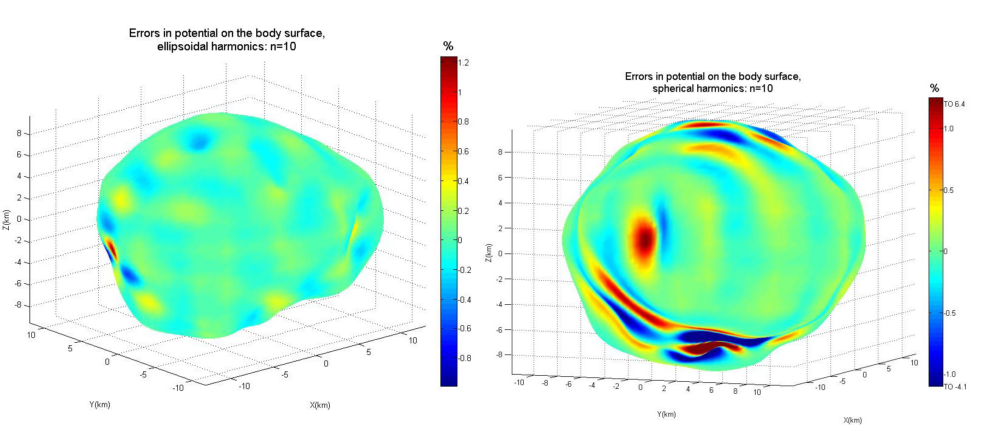
\includegraphics[width=\textwidth]{surface_comparison_spherical_ellipsoidal.png}
\caption{Difference in the computed gravitational potential for Phobos between the polyhedron model and the two harmonic, ellipsoidal (shown on the left) and spherical (shown on the right), expansion models \cite{spherical_ellipsoidal_comparison}.}
\label{fig:surface_comparison_spherical_ellipsoidal}
\end{figure}

% From computation point of view, in case of ellipsoidal harmonic expansion, one has to perform transformations between the ellipsoidal and Cartesian coordinates at each time step all the while ensuring that the constraints that ensure a unique one to one transformation between the two coordinate forms are not violated.
%
\begin{figure}[h]
\centering
\captionsetup{justification=centering}
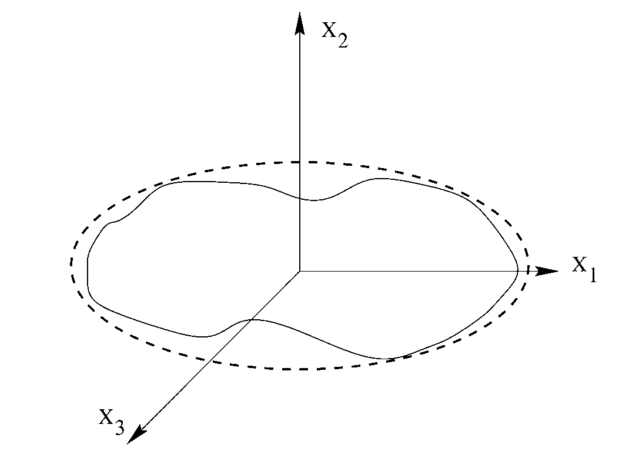
\includegraphics[scale=0.5]{circum_ellipsoid.png}
\caption{Circumscribing or Brillouin ellipsoid \cite{ellipse_main}.}
\label{fig:circum_ellip}
\end{figure}
\FloatBarrier
%

In general, for both spherical and ellipsoidal harmonics, a common drawback is that these models do not provide information on whether a field point (the point at which the gravitational potential is to be calculated) is inside or outside the body \cite{dan_poly}, an information which is very useful when designing orbits very close to the surface of an asteroid.

After the harmonic models, we shall now discuss the elliptic integral potential model wherein the body is assumed to be a perfect ellipsoid of constant density. The variant of ellipsoidal coordinates used in this model ensures that its transformation to Cartesian coordinate is one-to-one without imposing any extra rules or constraints. The integrals involved in the potential formula can be expressed as elliptic integrals of the first and the second kind in order to be evaluated. However the model presented in \Cref{elliptic_integral} has provided an alternate representation for these integrals allowing their evaluation by just using any numerical integration algorithm. This makes the computation of the elliptic integral potential model much easier than the harmonic expansion models. Unlike the harmonic expansion models, the elliptic integral model is not truncated at a certain degree or order and therefore the latter is more accurate than the former.

The mass concentrations or "mascons" model is easy to develop but is computationally intensive since at each time step the acceleration due to individual point masses has to be calculated. Although the model can be used to approximate the shape and density of a given asteroid to a great accuracy but for a given computational effort, the mascons approach is less accurate than the harmonics approach in its given region of convergence \cite{dan_poly}.

The final approach that we used to model the gravity field for an asteroid is by using a constant density polyhedron. Small details such as craters, elevations, slopes and other surface features can be included in modeling the asteroid with very high resolution. The biggest advantage of polyhedron modeling is that the potential is valid and exact for any given shape up to the surface of that body. Thus there are no regions of divergence, unlike that in the case of harmonic models, which means that close proximity orbits can be designed using the polyhedron potential. Errors in polyhedron potential modeling can arise because of errors in shape determination of an asteroid, the resolution selected for modeling i.e. the number of facets used to represent the polyhedron, and finally because of the assumption that the asteroid is of constant density \cite{ellipse_colorado}. Another drawback is that the computational effort required in this model is quite significant. Polyhedron models are generally helpful when considering the design of lander trajectories because it involves surface interaction and harmonic models will diverge if the potential is calculated at the surface of an irregular body. Also, polyhedron models restrict the orbit design strategy to be specific to the body being modeled and not to any arbitrary body.

After discussing all the pros and cons of the various potential models and for the application of studying the motion of lofted regolith from the surface of an asteroid, a study that will involve obtaining orbits close to the surface of the asteroid with a possibility for surface interaction, the polyhedron model will be the most suitable and hence it will be used for the thesis in future.


